\section{Tugas 3 -- Clustering Multimodal Material}
Data: 36.000 sampel tanpa label, masing-masing dengan citra mikrostruktur $64\times64$ dan spektrum komposisi 128 titik; dua mikroskop (M1, M2).

\subsection*{(a) Distorsi pada data}
\textbf{Gambar:} orientasi tekstur tersebar merata (rotasi acak), skala bervariasi, dan mikroskop M2 lebih terang (rata-rata \TtigaKecerahanMdua{} vs \TtigaKecerahanMsatu{} pada M1;
Gambar~\ref{fig:t3gambar} dan \ref{fig:t3distorsi}). \textbf{Spektrum:} posisi puncak bergeser beberapa titik, terdapat baseline miring/melengkung, dan \emph{spike} tunggal pada
\TtigaSpikePersen\% titik (\TtigaSpikeSpektrum\% spektrum). Preprocessing spektrum (Gambar~\ref{fig:t3prep}): spike dideteksi sebagai titik yang menyimpang jauh dari rata-rata dua
tetangganya lalu diganti; baseline polinomial derajat 2 di-fit ke ``lantai'' spektrum lalu dikurangkan; terakhir normalisasi SNV. Gambar distandarisasi per mikroskop.

\begin{figure}[ht]\centering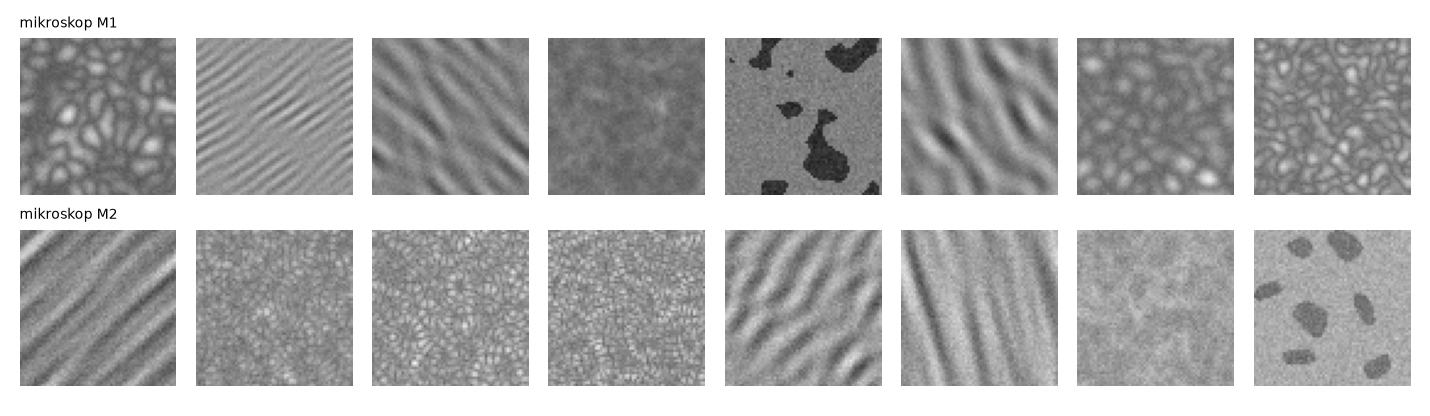
\includegraphics[width=\linewidth]{t3_eda_gambar.png}
\caption{Contoh citra mikrostruktur dari mikroskop M1 (atas) dan M2 (bawah).}\label{fig:t3gambar}\end{figure}
\begin{figure}[ht]\centering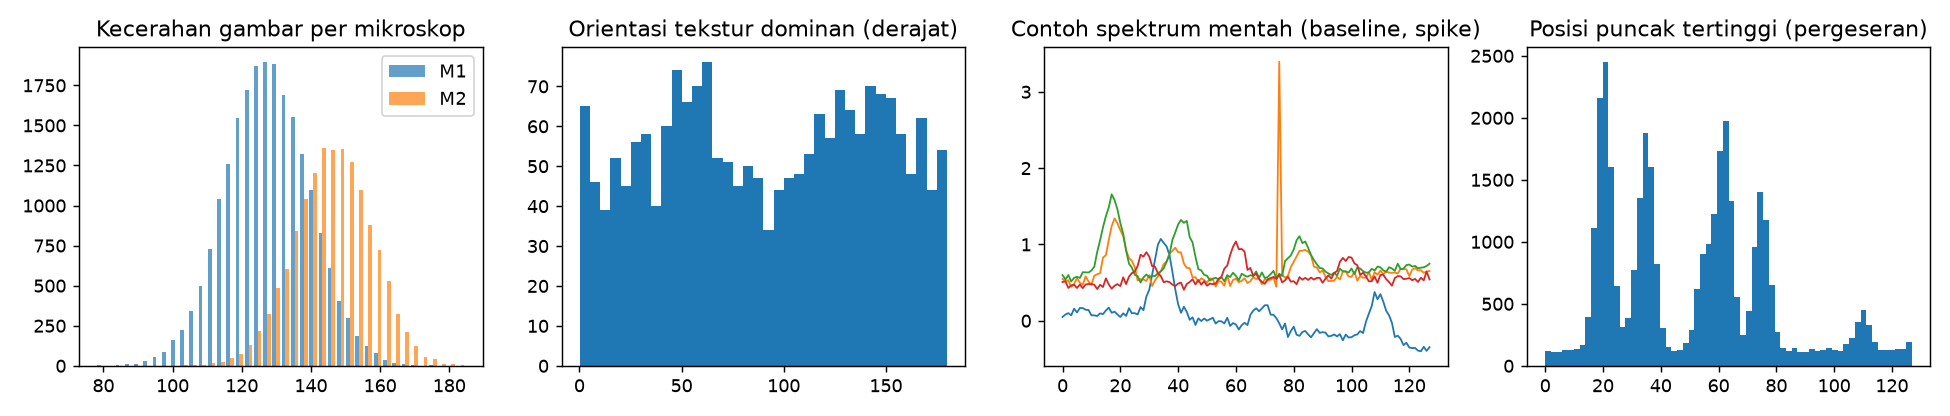
\includegraphics[width=\linewidth]{t3_eda_distorsi.png}
\caption{Kecerahan per mikroskop, orientasi tekstur, contoh spektrum mentah, dan posisi puncak.}\label{fig:t3distorsi}\end{figure}
\begin{figure}[ht]\centering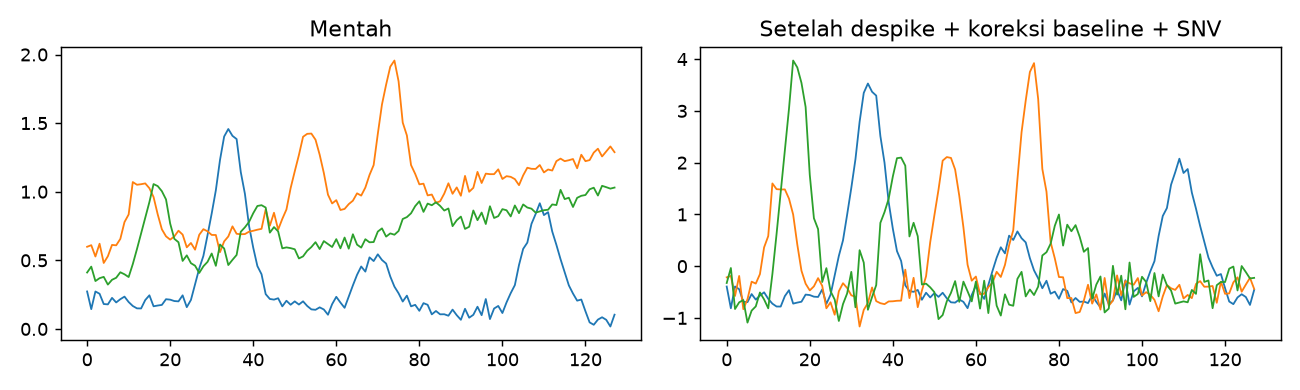
\includegraphics[width=.75\linewidth]{t3_preprocessing_spektrum.png}
\caption{Spektrum sebelum dan sesudah despike, koreksi baseline, dan SNV.}\label{fig:t3prep}\end{figure}

\subsection*{(b) Representasi tanpa label}
Dipakai \emph{SimCLR}: dua augmentasi acak dari sampel yang sama didekatkan dan sampel lain dijauhkan (loss NT-Xent, $\tau=0{,}2$). Augmentasi sengaja meniru
distorsi yang \emph{tidak} boleh memengaruhi tipe material, sehingga representasi menjadi invarian terhadapnya:
\begin{itemize}
  \item gambar: rotasi bebas $0$--$360^\circ$ dan flip (material tidak punya orientasi), skala $0{,}75$--$1{,}25$, kecerahan/kontras (beda mikroskop), blur dan noise;
  \item spektrum: geser $\pm4$ titik (pergeseran puncak), sisa baseline acak kuadratik, spike acak, noise, dan skala intensitas.
\end{itemize}
Encoder gambar adalah CNN yang sama dengan Tugas 1; encoder spektrum 1D-CNN tiga blok. Kurva loss ada di Gambar~\ref{fig:t3loss}.

\subsection*{(c) Dua modalitas}
Dua cara penggabungan dibandingkan: (i) \emph{concat} embedding SimCLR gambar dan spektrum yang dilatih terpisah, (ii) \emph{joint} gaya CLIP --- kedua encoder dilatih
bersama dengan SimCLR per modalitas \emph{ditambah} loss kontrastif lintas-modal (gambar dan spektrum dari sampel yang sama adalah pasangan positif).
PCA piksel+spektrum dilaporkan sebagai pembanding non-DL (Tabel~\ref{tab:t3_representasi}). Representasi gabungan terpilih: \textbf{\TtigaKonfigFusion}.
Dengan gambar saja terpilih $k=\TtigaKGambar$ dan dengan spektrum saja $k=\TtigaKSpektrum$. Kesesuaian cluster gabungan dengan cluster spektrum saja ARI \TtigaARIGabSpek{}
dan dengan gambar saja \TtigaARIGabGambar; crosstab di Gambar~\ref{fig:t3ct} menunjukkan cluster gabungan mana yang \emph{melebur} bila hanya satu modalitas dipakai.
Contoh pasangan yang hanya terpisah oleh gambar adalah cluster 3 dan 4 pada hasil akhir: puncak spektrum keduanya di posisi yang sama (62, Tabel~\ref{tab:t3_per_cluster}), sehingga pembedanya adalah tekstur mikrostruktur. Sebaliknya, pada run ini hampir tidak ada pasangan yang hanya terpisah oleh spektrum: setiap cluster dari gambar saja masuk ke satu cluster gabungan (ARI 0.900), sedangkan kesesuaian dengan cluster spektrum saja rendah (ARI 0.105). Artinya representasi gabungan masih didominasi gambar; ini menjadi keterbatasan sekaligus arah perbaikan, misalnya memberi bobot lebih besar pada loss lintas-modal.
\begin{table}[ht]
\centering\small
\resizebox{\ifdim\width>\linewidth\linewidth\else\width\fi}{!}{%
\begin{tabular}{lrrrr}
\toprule
representasi & k\_terpilih & silhouette & stabilitas\_ARI & ARI\_dengan\_mikroskop \\
\midrule
gambar saja (SimCLR) & 6 & 0.478 & 1.000 & -0.000 \\
spektrum saja (SimCLR) & 5 & 0.243 & 0.978 & -0.001 \\
gabungan concat & 5 & 0.304 & 0.927 & 0.000 \\
gabungan joint (CLIP) & 5 & 0.278 & 0.931 & 0.000 \\
PCA piksel+spektrum (pembanding non-DL) & 5 & 0.208 & 0.968 & 0.002 \\
\bottomrule
\end{tabular}
}
\caption{Representasi: k terpilih (aturan stabilitas $\geq$ 0.90 lalu silhouette tertinggi), kualitas, dan ARI dengan mikroskop.}
\label{tab:t3_representasi}
\end{table}

\begin{figure}[ht]\centering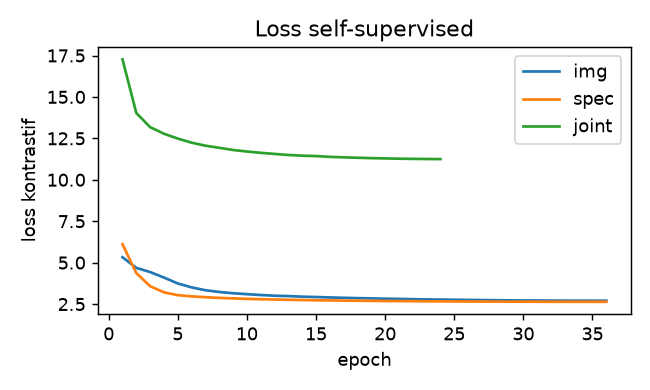
\includegraphics[width=.4\linewidth]{t3_ssl_loss.png}\hspace{1em}
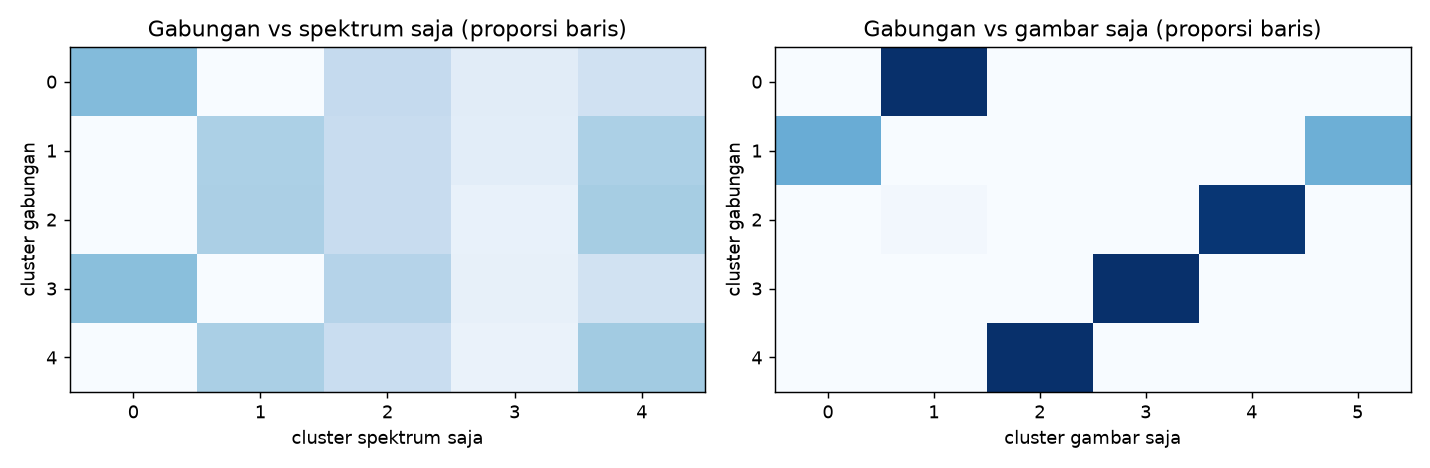
\includegraphics[width=.55\linewidth]{t3_crosstab_modalitas.png}
\caption{Kiri: loss self-supervised. Kanan: cluster gabungan vs cluster satu modalitas (proporsi baris).}\label{fig:t3loss}\label{fig:t3ct}\end{figure}

\subsection*{(d)--(e) Metode dan jumlah cluster}
Pada representasi terpilih, $k = 2,\dots,15$ dinilai dengan silhouette, stabilitas (rata-rata ARI antar 5 run subsampling 80\%), dan BIC GMM (Gambar~\ref{fig:t3k},
Tabel~\ref{tab:t3_kriteria_k}). Aturan yang ditetapkan sebelum melihat hasil: \emph{di antara $k \geq 3$ yang stabil (ARI $\geq 0{,}90$), pilih silhouette tertinggi}.
Terpilih $k = \TtigaK$ (silhouette \TtigaSilK, stabilitas \TtigaStabK). Empat metode dibandingkan pada $k$ tersebut (Tabel~\ref{tab:t3_metode}): K-Means, GMM diagonal,
Agglomerative Ward, dan \emph{DEC} (Deep Embedded Clustering: autoencoder kecil di atas embedding, centroid diinisialisasi K-Means, lalu dioptimasi dengan
KL antara soft assignment Student-$t$ dan distribusi target yang dipertajam). Terpilih \textbf{\TtigaKonfigMetode} (metode paling stabil antar seed).
ARI cluster akhir dengan mikroskop \TtigaARIMikroskopFinal{} $\approx 0$: cluster tidak sekadar memisahkan mikroskop.

\begin{figure}[ht]\centering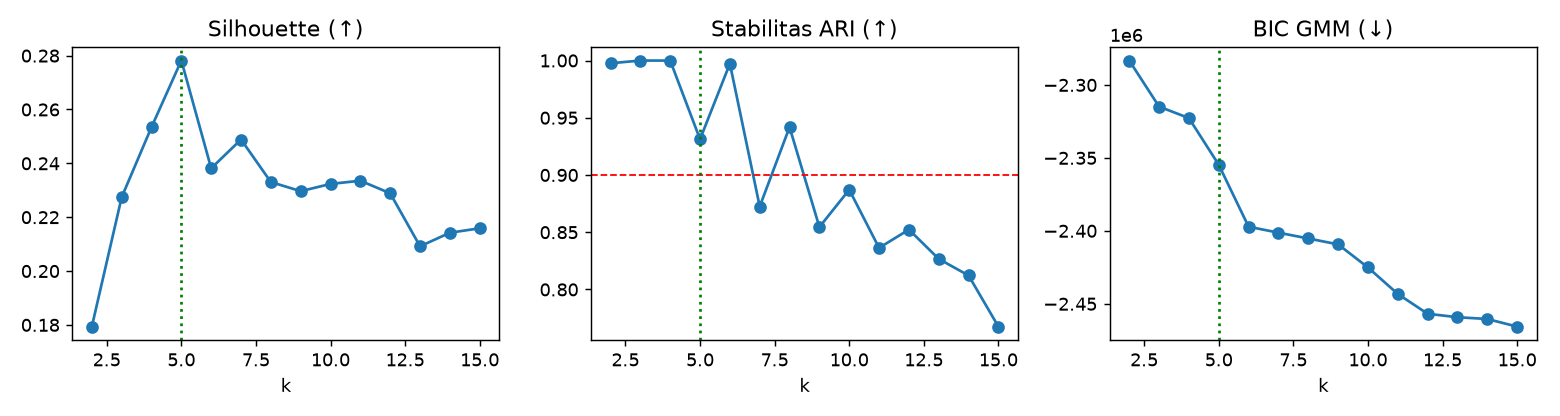
\includegraphics[width=\linewidth]{t3_kriteria_k.png}
\caption{Kriteria jumlah cluster; garis hijau = $k$ terpilih.}\label{fig:t3k}\end{figure}
\begin{table}[ht]
\centering\small
\resizebox{\ifdim\width>\linewidth\linewidth\else\width\fi}{!}{%
\begin{tabular}{rrrrrrr}
\toprule
k & silhouette & davies\_bouldin & bic\_gmm & stabilitas\_ARI & stabilitas\_min & ukuran\_terkecil\_\% \\
\midrule
2 & 0.179 & 2.070 & -2283282.303 & 0.998 & 0.995 & 42.475 \\
3 & 0.227 & 1.837 & -2314852.422 & 1.000 & 1.000 & 24.164 \\
4 & 0.253 & 1.609 & -2322737.164 & 1.000 & 1.000 & 10.156 \\
5 & 0.278 & 1.490 & -2354728.242 & 0.931 & 0.828 & 10.156 \\
6 & 0.238 & 1.484 & -2397181.438 & 0.997 & 0.996 & 10.156 \\
7 & 0.249 & 1.552 & -2401260.713 & 0.872 & 0.770 & 10.156 \\
8 & 0.233 & 1.616 & -2405238.634 & 0.942 & 0.863 & 10.156 \\
9 & 0.230 & 1.541 & -2409291.014 & 0.855 & 0.764 & 7.347 \\
10 & 0.232 & 1.519 & -2425091.265 & 0.887 & 0.825 & 6.667 \\
11 & 0.234 & 1.503 & -2443261.555 & 0.836 & 0.722 & 4.961 \\
12 & 0.229 & 1.492 & -2456844.745 & 0.852 & 0.731 & 4.961 \\
13 & 0.209 & 1.598 & -2459216.140 & 0.827 & 0.694 & 4.936 \\
14 & 0.214 & 1.573 & -2460424.780 & 0.812 & 0.721 & 3.003 \\
15 & 0.216 & 1.593 & -2465670.483 & 0.768 & 0.698 & 4.961 \\
\bottomrule
\end{tabular}
}
\caption{Kriteria jumlah cluster pada representasi terpilih (gabungan joint (CLIP)).}
\label{tab:t3_kriteria_k}
\end{table}

\begin{table}[ht]
\centering\small
\resizebox{\ifdim\width>\linewidth\linewidth\else\width\fi}{!}{%
\begin{tabular}{lrrrrr}
\toprule
metode & silhouette & ARI\_antar\_seed & ARI\_vs\_KMeans & ARI\_dengan\_mikroskop & ukuran\_terkecil\_\% \\
\midrule
K-Means & 0.278 & 0.828 & 1.000 & 0.000 & 10.156 \\
GMM (diag) & 0.278 & 1.000 & 0.992 & 0.000 & 10.156 \\
Agglomerative Ward & 0.278 & 1.000 & 0.999 & 0.000 & 10.156 \\
DEC (deep clustering) & 0.202 & 0.567 & 0.560 & 0.000 & 16.964 \\
\bottomrule
\end{tabular}
}
\caption{Perbandingan metode clustering pada k = 5.}
\label{tab:t3_metode}
\end{table}


\subsection*{(f) Analisis}
t-SNE pada 5.000 sampel (Gambar~\ref{fig:t3tsne}) menunjukkan \TtigaNCluster{} kelompok dan tidak ada pemisahan menurut mikroskop. Ringkasan per cluster
(silhouette, porsi tetangga dari cluster lain, posisi puncak spektrum) ada di Tabel~\ref{tab:t3_per_cluster}; contoh gambar dan spektrum rata-rata di Gambar~\ref{fig:t3contoh}.
Pasangan yang paling sulit dipisah (tetangga terdekat paling sering bercampur) adalah cluster \TtigaSulitA{} dan \TtigaSulitB.
Meski disebut ``paling sulit'', pencampurannya sangat kecil: hanya 0.24\% tetangga terdekat cluster 0 dan 3 berasal dari cluster pasangannya. Puncak spektrum keduanya berbeda (posisi 20 vs 62), sehingga keduanya berdekatan karena tekstur citranya mirip, bukan karena komposisinya sama (Gambar~\ref{fig:t3contoh}). Cluster dengan silhouette terendah justru cluster 2 (0.18), yang menunjukkan materialnya paling bervariasi di dalam kelompoknya.  
\begin{figure}[ht]\centering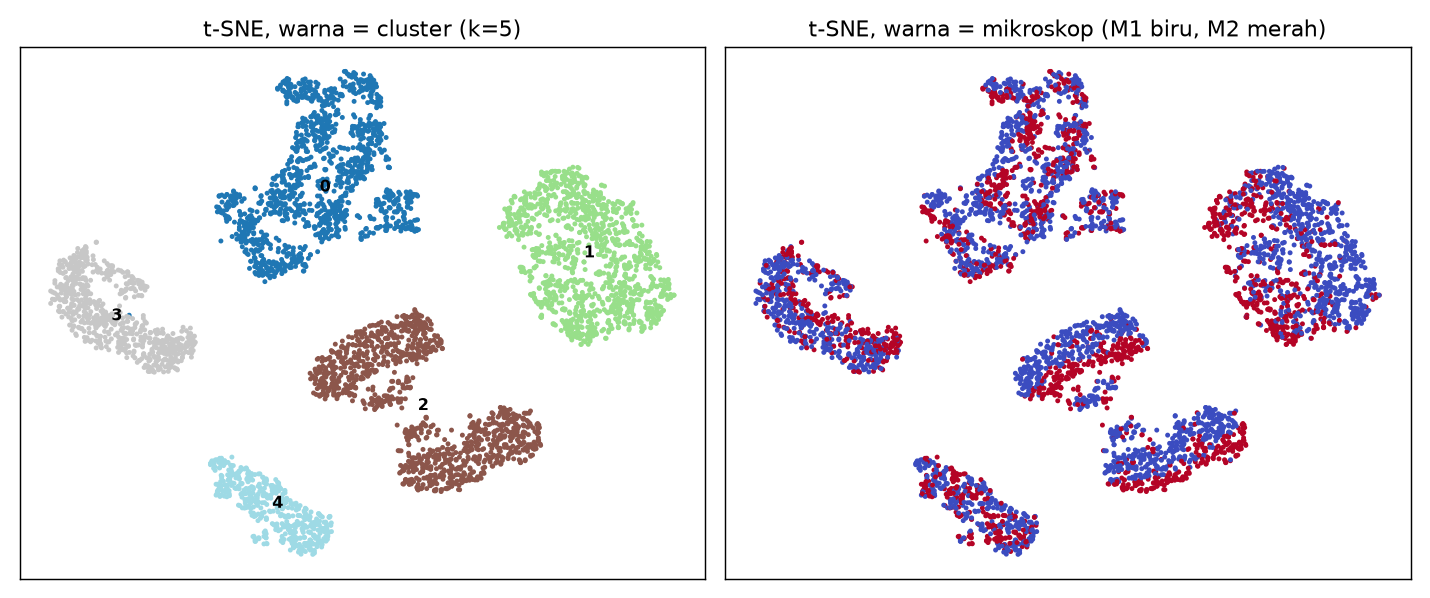
\includegraphics[width=.95\linewidth]{t3_tsne.png}
\caption{t-SNE embedding gabungan: warna menurut cluster (kiri) dan mikroskop (kanan).}\label{fig:t3tsne}\end{figure}
\begin{table}[ht]
\centering\small
\resizebox{\ifdim\width>\linewidth\linewidth\else\width\fi}{!}{%
\begin{tabular}{rrrrrr}
\toprule
cluster & ukuran\_\% & silhouette\_rata2 & porsi\_M2\_\% & tetangga\_beda\_cluster\_\% & posisi\_puncak\_spektrum \\
\midrule
0 & 27.93 & 0.29 & 40.11 & 0.07 & 20 \\
1 & 24.12 & 0.30 & 39.15 & 0.02 & 75 \\
2 & 23.99 & 0.18 & 39.98 & 0.07 & 35 \\
3 & 13.80 & 0.33 & 40.05 & 0.17 & 62 \\
4 & 10.16 & 0.35 & 40.70 & 0.00 & 62 \\
\bottomrule
\end{tabular}
}
\caption{Ringkasan tiap cluster: ukuran, silhouette, porsi mikroskop M2, tetangga terdekat dari cluster lain, posisi puncak spektrum.}
\label{tab:t3_per_cluster}
\end{table}

\begin{figure}[ht]\centering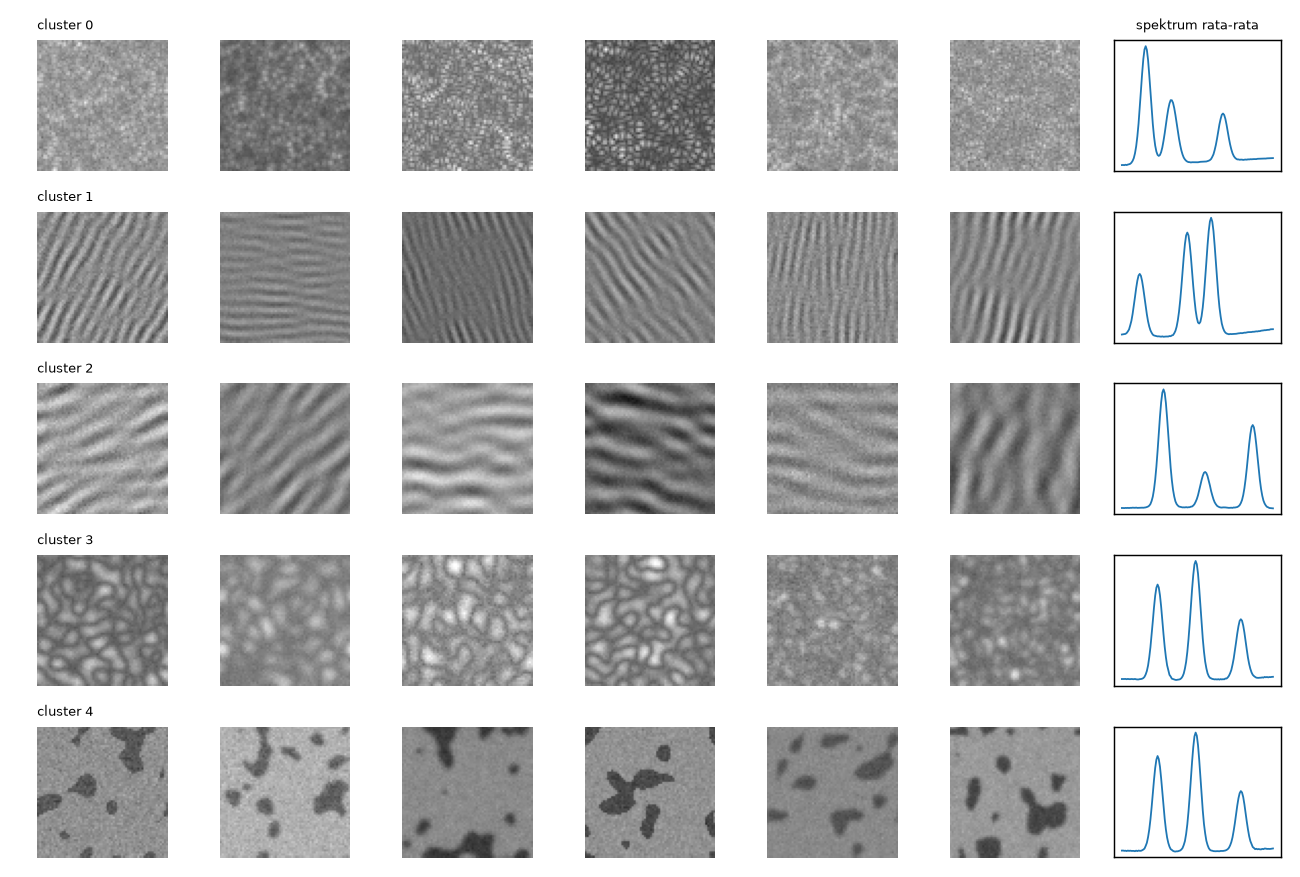
\includegraphics[width=.75\linewidth]{t3_contoh_cluster.png}
\caption{Contoh gambar dan spektrum rata-rata tiap cluster.}\label{fig:t3contoh}\end{figure}
